\chapter*{}

%$ \ddot{x} \quad 	\displaystyle \dot{x} \quad  \va*{a} \quad \fdv{g} \quad \fdv{F}{g} \quad \fdv{V}(E-TS) \quad  \fdv*{F}{x}$

La \emph{mecánica clásica} es la rama de la física que estudia las leyes del comportamiento de cuerpos físicos macroscópicos (a diferencia de la mecánica cuántica) en reposo y a velocidades pequeñas comparadas con la velocidad de la luz (mecánica relativista).

En la mecánica clásica en general se tienen tres aspectos invariantes: el tiempo es absoluto, la naturaleza realiza de forma espontánea la mínima acción y la concepción de un universo determinado.


El primer desarrollo de la mecánica clásica suele denominarse \emph{mecánica newtoniana}. Consiste en los conceptos físicos basados en los trabajos fundacionales de Sir Isaac Newton, y en los métodos matemáticos inventados por Gottfried Wilhelm Leibniz, Joseph-Louis Lagrange, Leonhard Euler, y otros contemporáneos, en el siglo XVII para describir el movimiento de los cuerpos físicos bajo la influencia de un sistema de fuerzas. Posteriormente, se desarrollaron métodos más abstractos que dieron lugar a las reformulaciones de la mecánica clásica conocidas como \emph{mecánica lagrangiana} y \emph{mecánica hamiltoniana}. Estos avances, realizados predominantemente en los siglos XVIII y XIX, van sustancialmente más allá de los trabajos anteriores, sobre todo por su uso de la mecánica analítica. También se utilizan, con algunas modificaciones, en todas las áreas de la física moderna.

La mecánica clásica proporciona resultados extremadamente precisos cuando se estudian objetos grandes que no son extremadamente masivos y velocidades que no se acercan a la velocidad de la luz. Cuando los objetos que se examinan tienen el tamaño del diámetro de un átomo, se hace necesario introducir el otro gran subcampo de la mecánica: la mecánica cuántica. Para describir las velocidades que no son pequeñas en comparación con la velocidad de la luz, se necesita la relatividad especial. En los casos en los que los objetos se vuelven extremadamente masivos, se aplica la relatividad general. Sin embargo, algunas fuentes modernas incluyen la mecánica relativista en la física clásica, que en su opinión representa la mecánica clásica en su forma más desarrollada y precisa.

Existen varias formulaciones diferentes, en mecánica clásica, para describir un mismo fenómeno natural que, independientemente de los aspectos formales y metodológicos que utilizan, llegan a la misma conclusión.

La \emph{mecánica vectorial}, que deviene directamente de las leyes de Newton, por lo que también se le conoce como ``mecánica newtoniana'', llega, a partir de las tres ecuaciones formuladas por Newton y mediante el cálculo diferencial e integral, a una muy exacta aproximación de los fenómenos físicos. Es aplicable a cuerpos que se mueven en relación con un observador a velocidades pequeñas comparadas con la de la luz. Fue construida en un principio para una sola partícula moviéndose en un campo gravitatorio. Se basa en el tratamiento de dos magnitudes vectoriales bajo una relación causal: la fuerza y la acción de la fuerza, medida por la variación del momentum (cantidad de movimiento). El análisis y síntesis de fuerzas y momentos constituye el método básico de la mecánica vectorial. Requiere del uso privilegiado de sistemas de referencia inercial

La \emph{mecánica analítica} es una formulación matemática abstracta sobre la mecánica; permite desligarse de esos sistemas de referencia privilegiados y tener conceptos más generales al momento de describir un movimiento con el uso del cálculo de variaciones. Sus métodos son poderosos y trascienden de la mecánica a otros campos de la física. Se puede encontrar el germen de la mecánica analítica en la obra de Leibniz, quien propone que para solucionar problemas en mecánica, magnitudes escalares (menos oscuras según Leibniz que la fuerza y el momento de Newton), como energía cinética y el trabajo, son suficientes y menos oscuras que las cantidades vectoriales, como la fuerza y el momento, propuestos por Newton. Existen dos formulaciones equivalentes: la llamada \emph{mecánica lagrangiana} es una reformulación de la mecánica realizada por \emph{Joseph Louis Lagrange} que se basa en la ahora llamada ecuación de Euler-Lagrange (ecuaciones diferenciales de segundo orden) y el principio de mínima acción; la otra, llamada \emph{mecánica hamiltoniana}, es una reformulación más teórica basada en una funcional llamada hamiltoniano realizada por \emph{William Hamilton}. Las mecánicas hamiltoniana y lagrangiana son ejemplos de mecánicas analíticas, donde las magnitudes se relacionan entre sí por ecuaciones diferenciales parciales.\footnote{Fuente: wikipedia.}

\rule{250pt}{0.1pt}

Establecer las fuerzas reales que actúan en un problema puede llegar a ser bastante complicado, sobre todo si existen \emph{ligaduras} que limitan el rango de una o varias variables. Además, las \emph{ecuaciones de Newton} cambian de forma y no son invariables ante transformaciones de coordenadas (rotaciones, traslaciones, …).

Las formulaciones \emph{lagrangiana} y \emph{hamiltoniana} se crearon para resolver estas dificultades y proporcionar un aparato matemático más poderoso con el que enfrentarse a los problemas mecánicos.

\vspace{1cm}

\textbf{Estructura}

\begin{adjustwidth}{20pt}{20pt}
	\vspace{5mm} \begin{myblock}{Teoría destacada}
		
	\end{myblock}
	
	\vspace{5mm} \begin{myalertblock}{Resultados destacados}
		
	\end{myalertblock}
	
	\vspace{5mm} \begin{ejemplo} 
		\textbf{Aclaraciones de Javier García}, normalmente al final del capítulo.
		
		\textbf{Introducciones a cada tema}, al inicio de cada capítulo.
	\end{ejemplo}
	
	
	\vspace{5mm} \begin{myexampleblock}{Aclaraciones, curiosidades, ...}
		
	\end{myexampleblock}
	
		\vspace{5mm} \begin{ejercicio} \textbf{Ejercicios propuestos.} \end{ejercicio}

\end{adjustwidth}





\vspace{1cm}

\centering{
\fcolorbox{black}{fondoblau}{
\parbox{0.95\textwidth}{
	\textit{Este material es un conjunto de apuntes personales que comparto gratuitamente en la red. Se agradecería la comunicación de la detección de cualquier error.}
}}}
\justify


Basado en los vídeo cursos de física de Javier García Garrido, licenciado en Física y Máster en Gravitación y Partículas, en este caso en el de ``Mecánica Teórica'':

\begin{center} \textcolor{blue}{https://www.youtube.com/playlist?list=PLAnA8FVrBl8C-2TTrbArT1g04RJEckRMG} \end{center}




\emph{\normalsize{Este} documento se comparte bajo licencia `Attribution-NonCommercial 4.0 International (CC BY-NC 4.0)'}


\begin{multicols}{2}
\begin{figure}[H]
	\centering
	
\includegraphics[width=.4
	\textwidth]{imagenes/licencia.png}
	
\end{figure}
\begin{figure}[H]
	\centering
	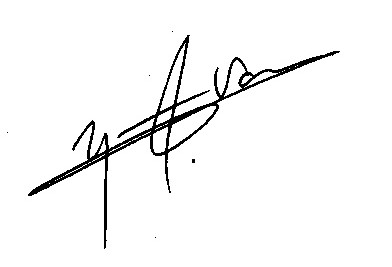
\includegraphics[width=.3
	\textwidth]{imagenes/firma.png}
\end{figure}
\end{multicols}

\newpage




\newpage

$\,$

\newpage

$\,$

\vspace{1cm} 

$\,$

\begin{figure}[H]
	\centering
	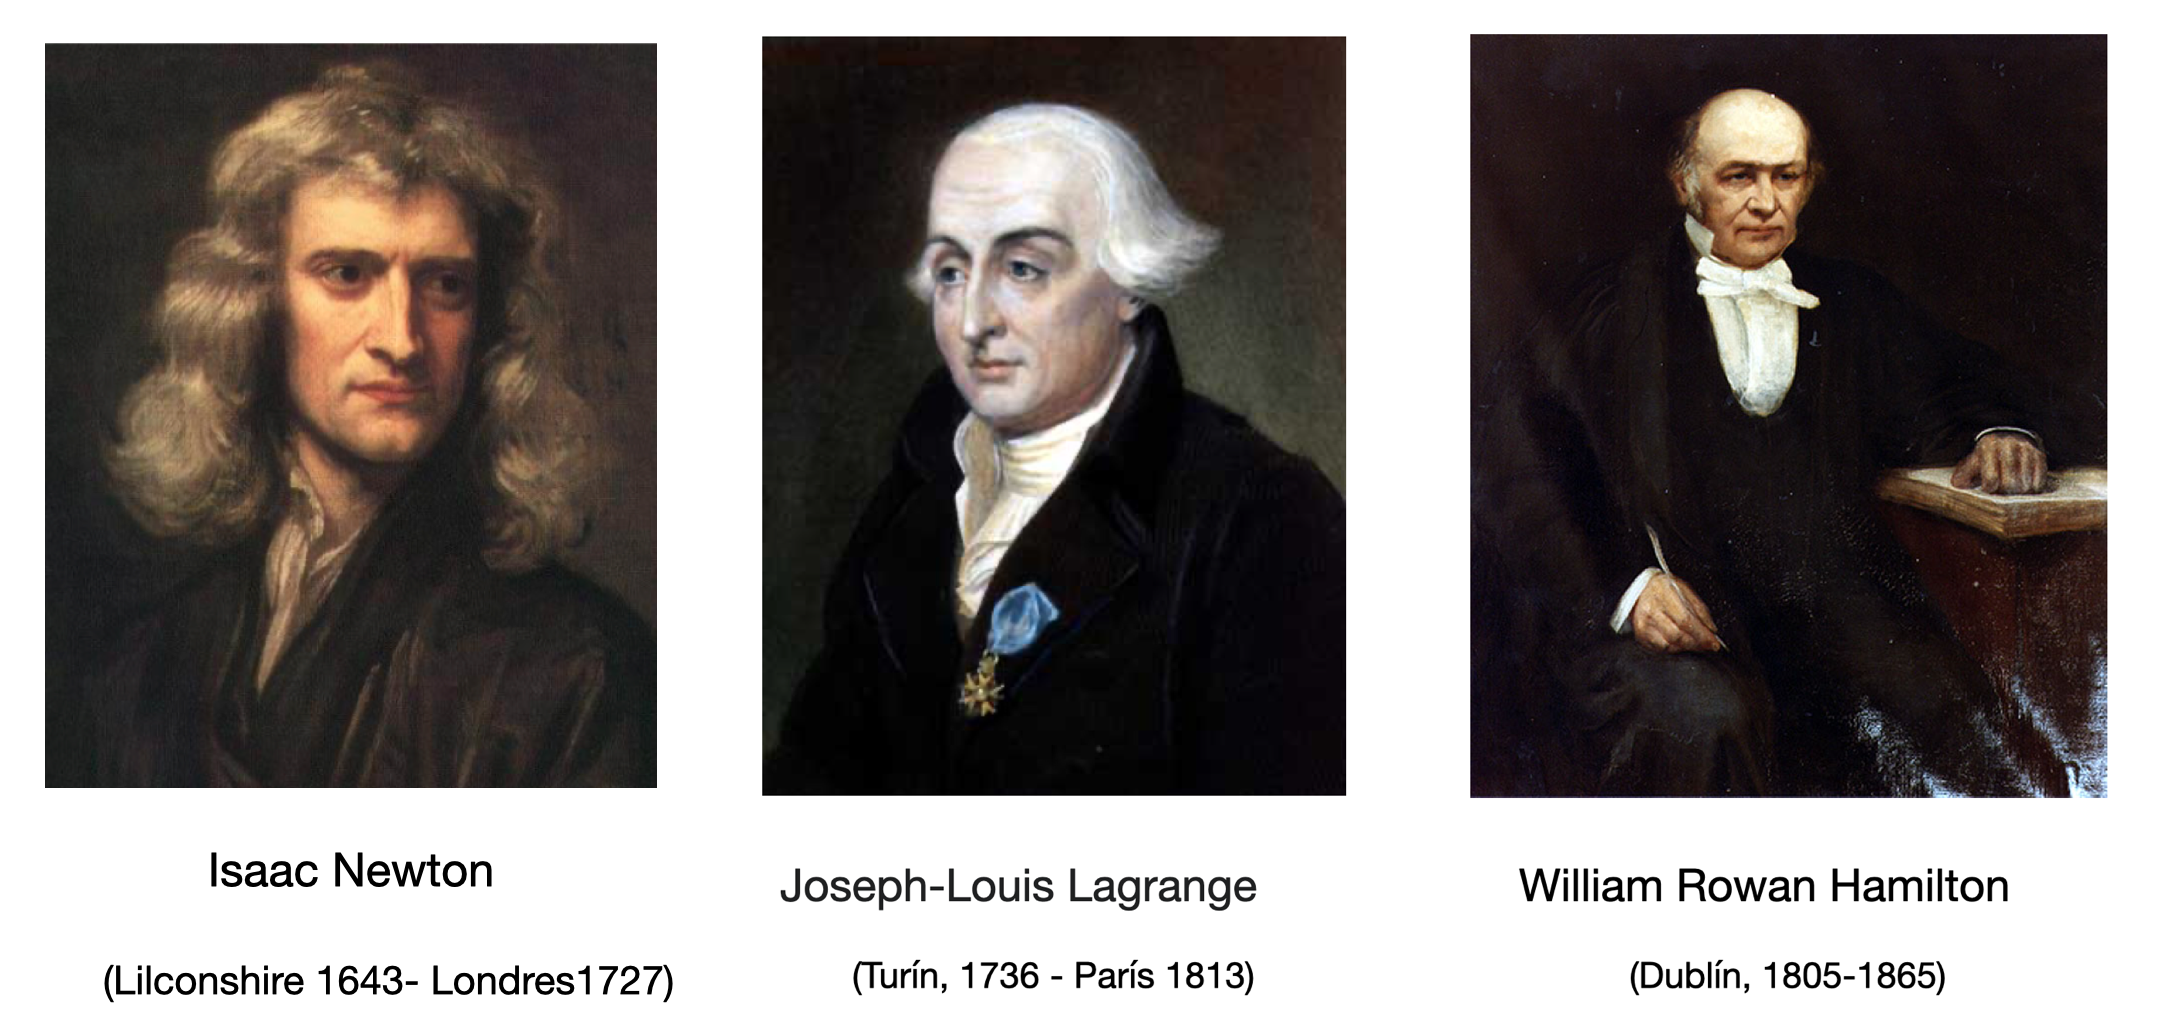
\includegraphics[width=.75\textwidth]{imagenes/portada.png}
\end{figure}


\begin{center}

\Huge{\textbf{Elementos clave de}}

\Huge{\textbf{Mecánica Teórica}} 


\large{\textbf{\textit{Video curso de Javier garcía}}}

\vspace{10mm}
\begin{figure}[H]
	\centering
	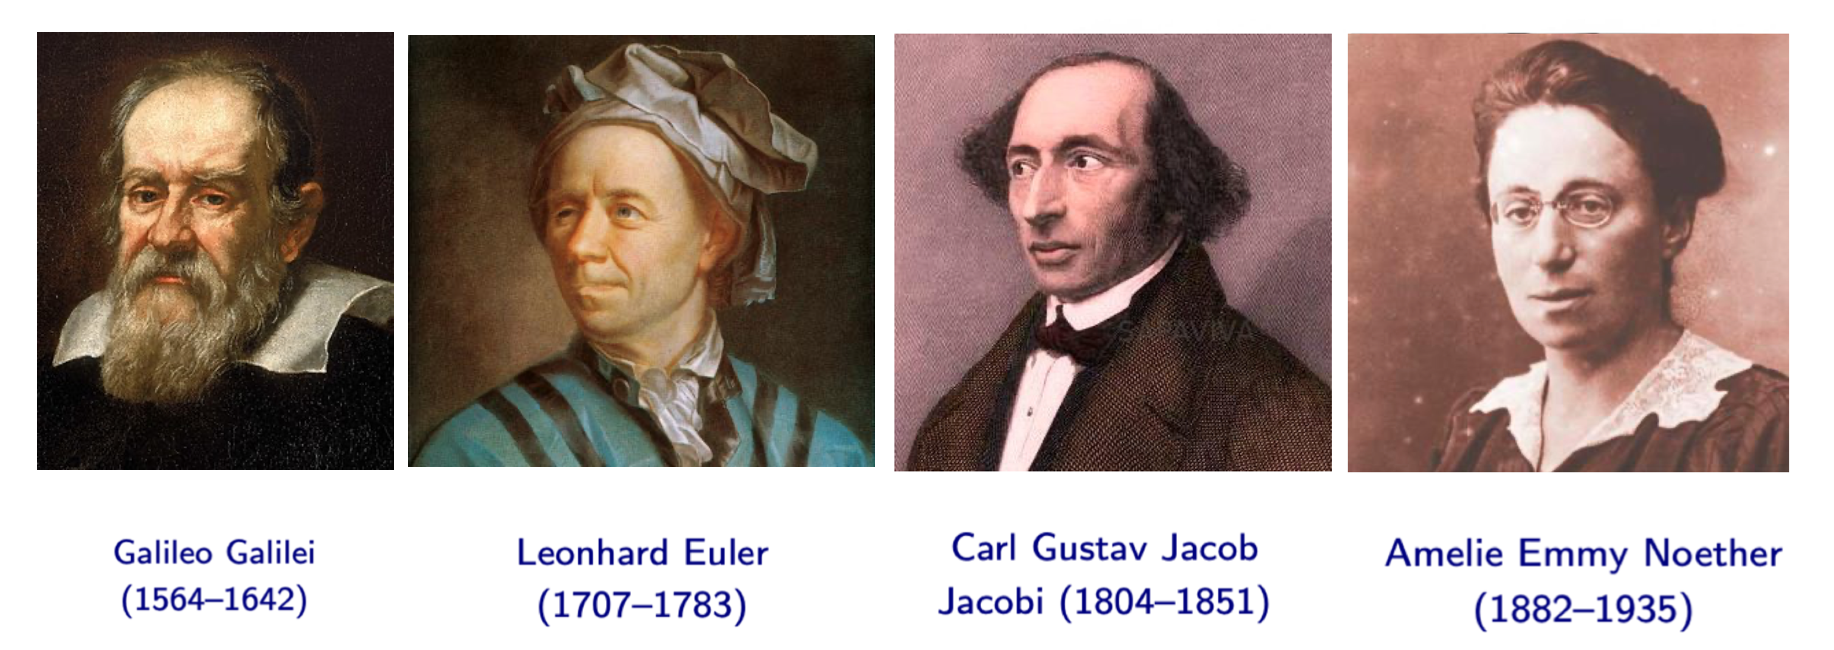
\includegraphics[width=.75\textwidth]{imagenes/portada2.png}
\end{figure}

\vspace{2cm}
\begin{flushright}
	\normalsize{\emph{Ignacio Vallés Oriola}}
\end{flushright}


\end{center}





